\chapter{Physical characterisation of few-layered 1T' $WSe_2$}

\section{Introduction}

The 1T and 1T' phases of group VI TMDCs have only recently gained significant attention compared to the more popular semiconducting 2H and number of reports in the literature has increased. They have been found to show promise in areas of electrocatalytic water splitting and energy storage thanks to lower charge transfer resistance \cite{Voiry2013}, a result of their metallic nature \cite{Wypych1992}. The 1T' phase is also predicted to be a large gap quantum spin Hall (QSH) insulator which can be useful in spintronic devices  application \cite{Chen2018}. In contrast to 1T' $WTe_2$ \cite{Fei2017} 1T' $WSe_2$ can be used in ambient temperatures as well as ambient atmosphere unlike other known large gap QSH insulator materials like stanene \cite{Xu2013} or 2D In-Sb compounds \cite{Gruznev2018}. 

So far the synthesis of 1T and 1T' group VI sulfides and selenides ($MoS_2$, $WS_2$, $MoSe_2$, $WSe_2$)  phases has proven difficult due to the metastable nature of them. Most commonly a direct synthesis via e.g. a CVD route results in more thermodynamically stable 2H phase. The difference in energy per formula unit between 1H and 1T' $WSe_2$ phase is only 0.27 eV which suggests that under certain reaction conditions a metastable 1T' can be synthesised.

The following work shows first time colloidal synthesis route of 1T' $WSe_2$ as well as Raman and XPS studies of the as grown material. The $WSe_2$ flakes of varying thickness has been successfully grown via the colloidal synthesis method by a fellow PhD student Maria Sokolikova.

\section{Results}

The sample was characterised using TEM as seen in Figure \ref{fig:1T'TEMMaps}. The TEM images show well defined flower shaped nanostructures with the average diameter of 200 nm. The petals stem from the central point and thin down towards the edges down to single layer. The single petals appear to be of 1T' phase while each petal is a single crystal. Additionally the structural parameters a = 5.76 \r{A} and b = 3.30 \r{A} have been identified. Reciprocal lattice created by FFT from high resolution TEM image from a single petal is rectangular and corresponding to monoclinic phase of $WSe_2$.

\begin{figure}[H]
	\begin{center}
		\begin{subfigure}[b]{0.4\textwidth}
			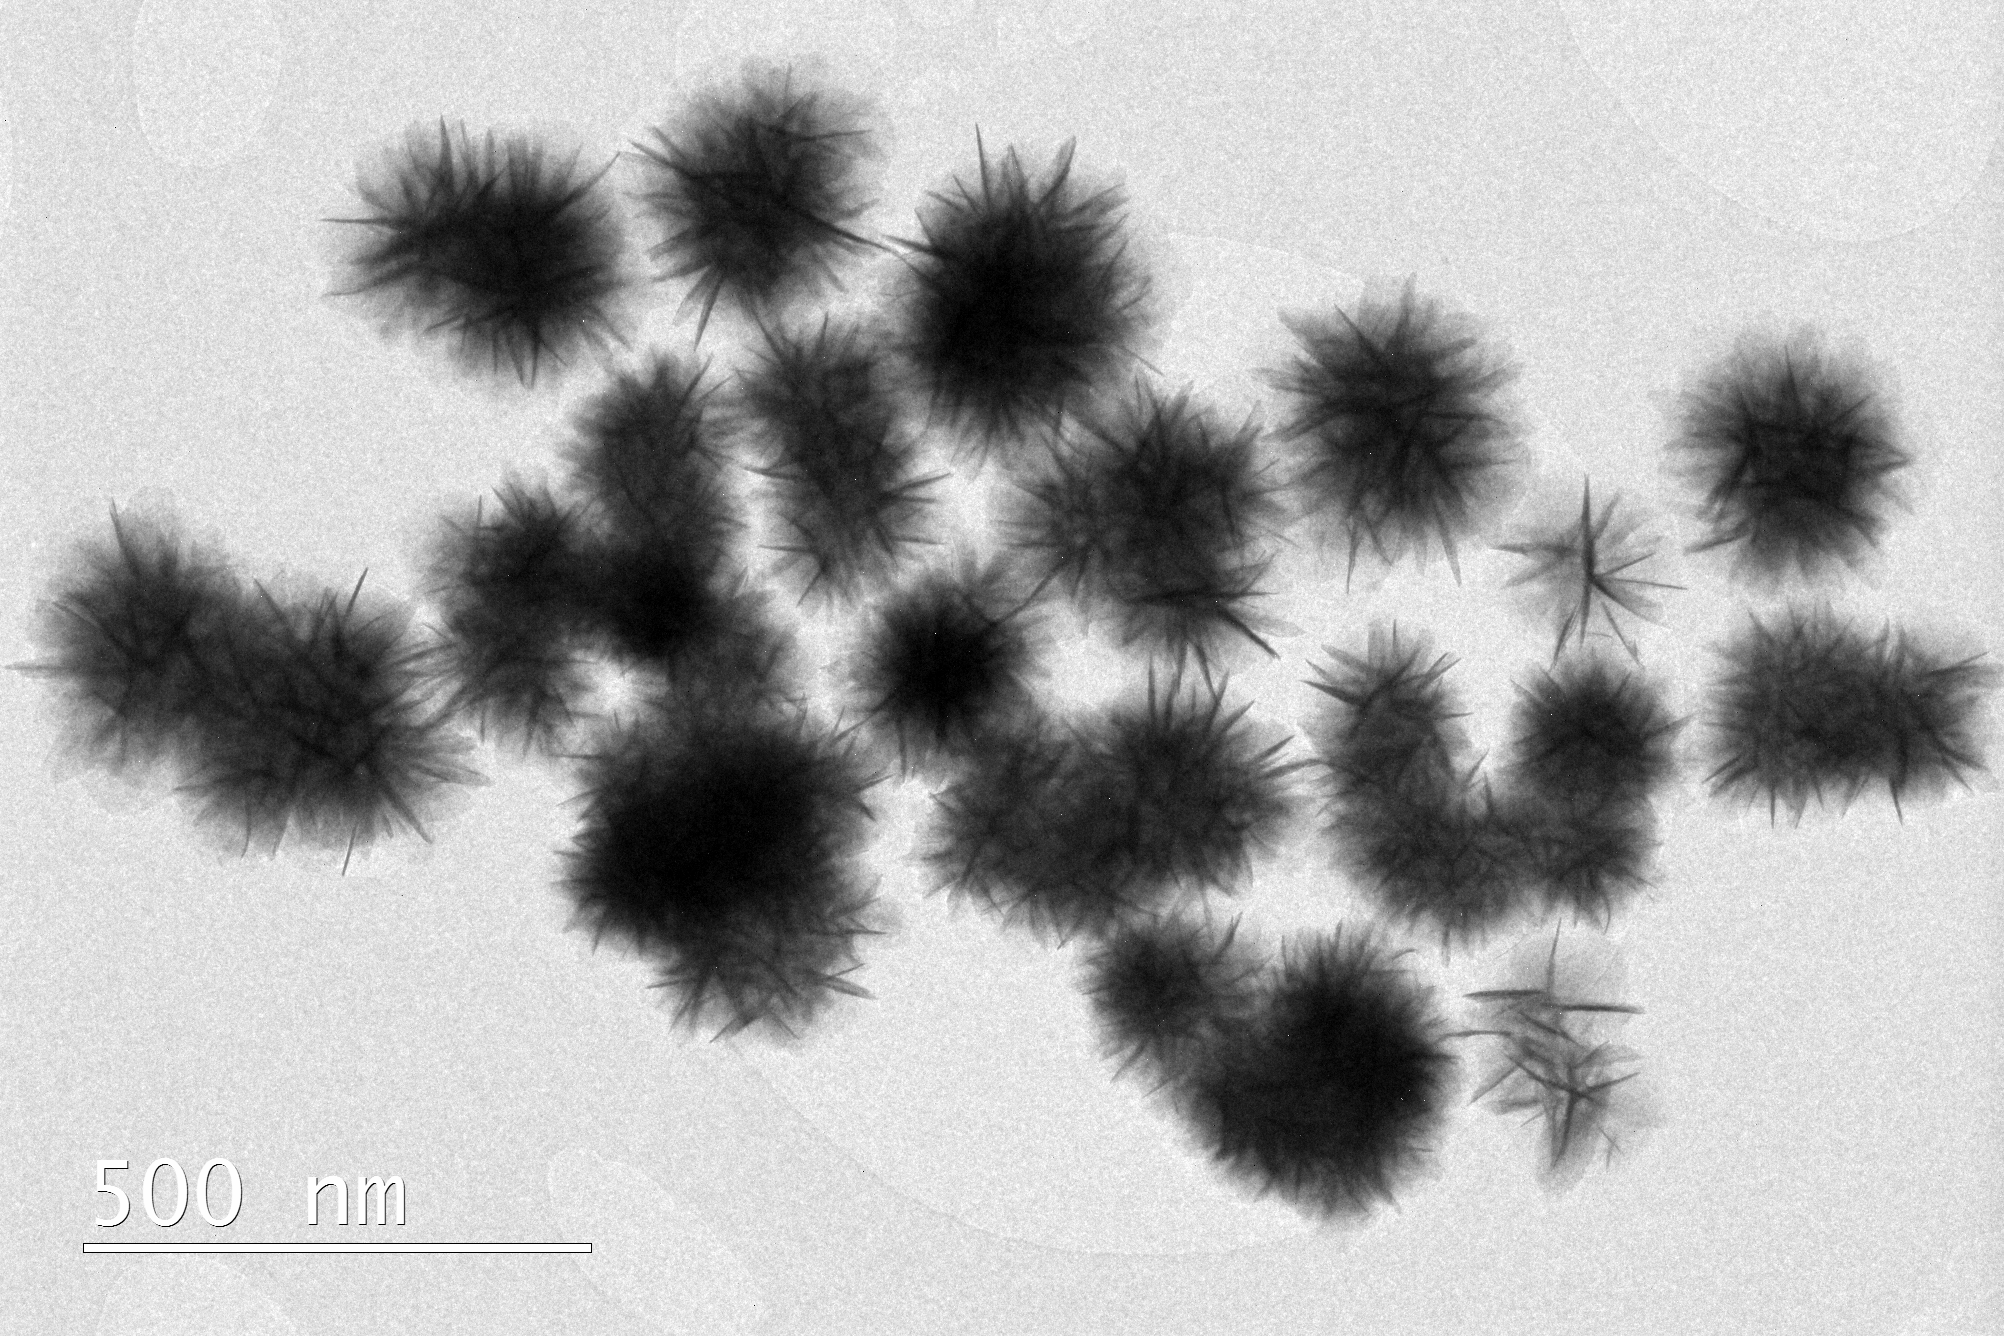
\includegraphics[width=\textwidth]{1T'/TEMImage.png}
			\caption{TEM image of as grown 1T' $WSe_2$ flakes.}
			\label{fig:1T'TEMImage}
		\end{subfigure}
		\qquad
		\begin{subfigure}[b]{0.4\textwidth}
			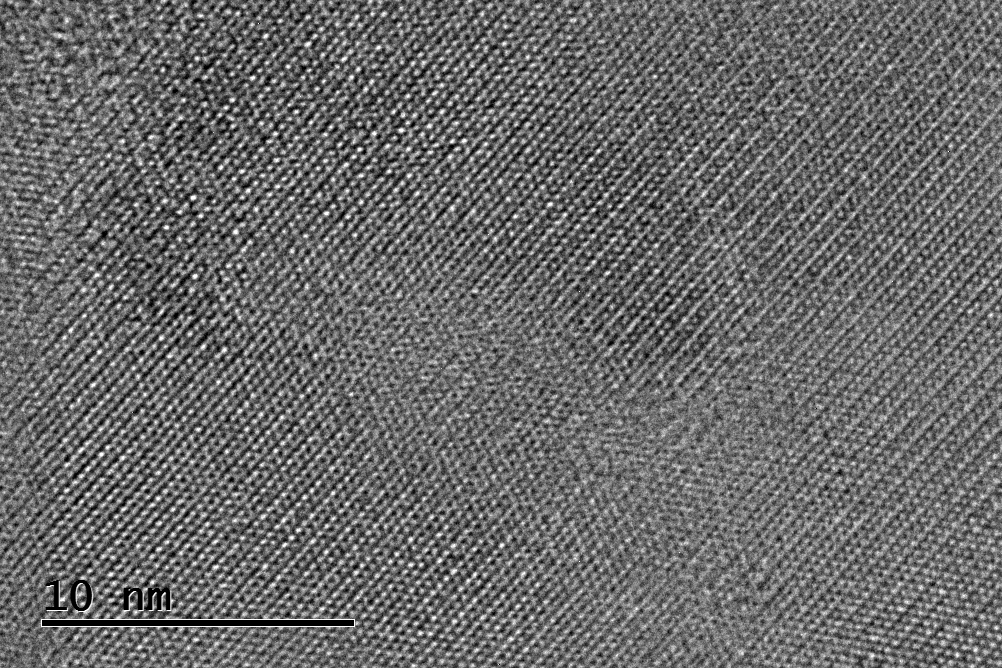
\includegraphics[width=\textwidth]{1T'/TEMImageHigh.png}
			\caption{High resolution TEM image.}
			\label{fig:1T'TEMImageHigh}
		\end{subfigure}
		\begin{subfigure}[b]{0.4\textwidth}
			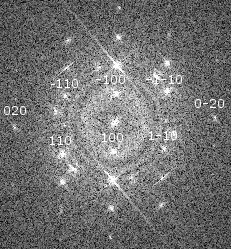
\includegraphics[width=\textwidth]{1T'/TEMEDFFT.png}
			\caption{FFT pattern constructed from the image in b).}
			\label{fig:1T'TEMEDFET}
		\end{subfigure}
		\caption{TEM characterisation of as grown 1T' flakes.}
		\label{fig:1T'TEMMaps}
	\end{center}
\end{figure}

In order to ascertain the phase of the as grown $WSe_2$ a Raman spectrum has been taken. As seen in Figure \ref{fig:1T'RamanSpectraComparison} the spectrum of the as grown 1T' $WSe_2$ looks very different to the Raman spectrum of the CVD grown 2H $WSe_2$ as seen in e.g. Figure \ref{fig:WSe2RamanSpectrum}. The $E^1_{2g}$ and $A_{1g}$ located around 250 $cm^{-1}$ and are convoluted in case of the monolayer. In spectrum of the 1T' sample (Figure \ref{fig:1T'RamanSpectraComparison}) the closest peaks to those are located at 248.6 and 260 $cm^{-1}$ and can be therefore ascribed to $E^1_{2g}$ and $A_{1g}$ modes respectively. Additionally the absence of the $B^1_{2g}$ peak suggest that the material is very thin. Furthermore there are 5 more unresolved peaks at 104.5, 149, 177, 218 and 236.3 $cm^{-1}$. Thus far there is no published information regarding the vibrational modes of 1T' $WSe_2$ and therefore the peaks cannot be assigned to the modes. Similarly new peaks have been reported for 1T' $MoS_2$ where new peaks were labelled as $J_1$, $J_2$ and $J_3$ \cite{Yu2018}.

\begin{figure}[!h]
	\begin{center}
		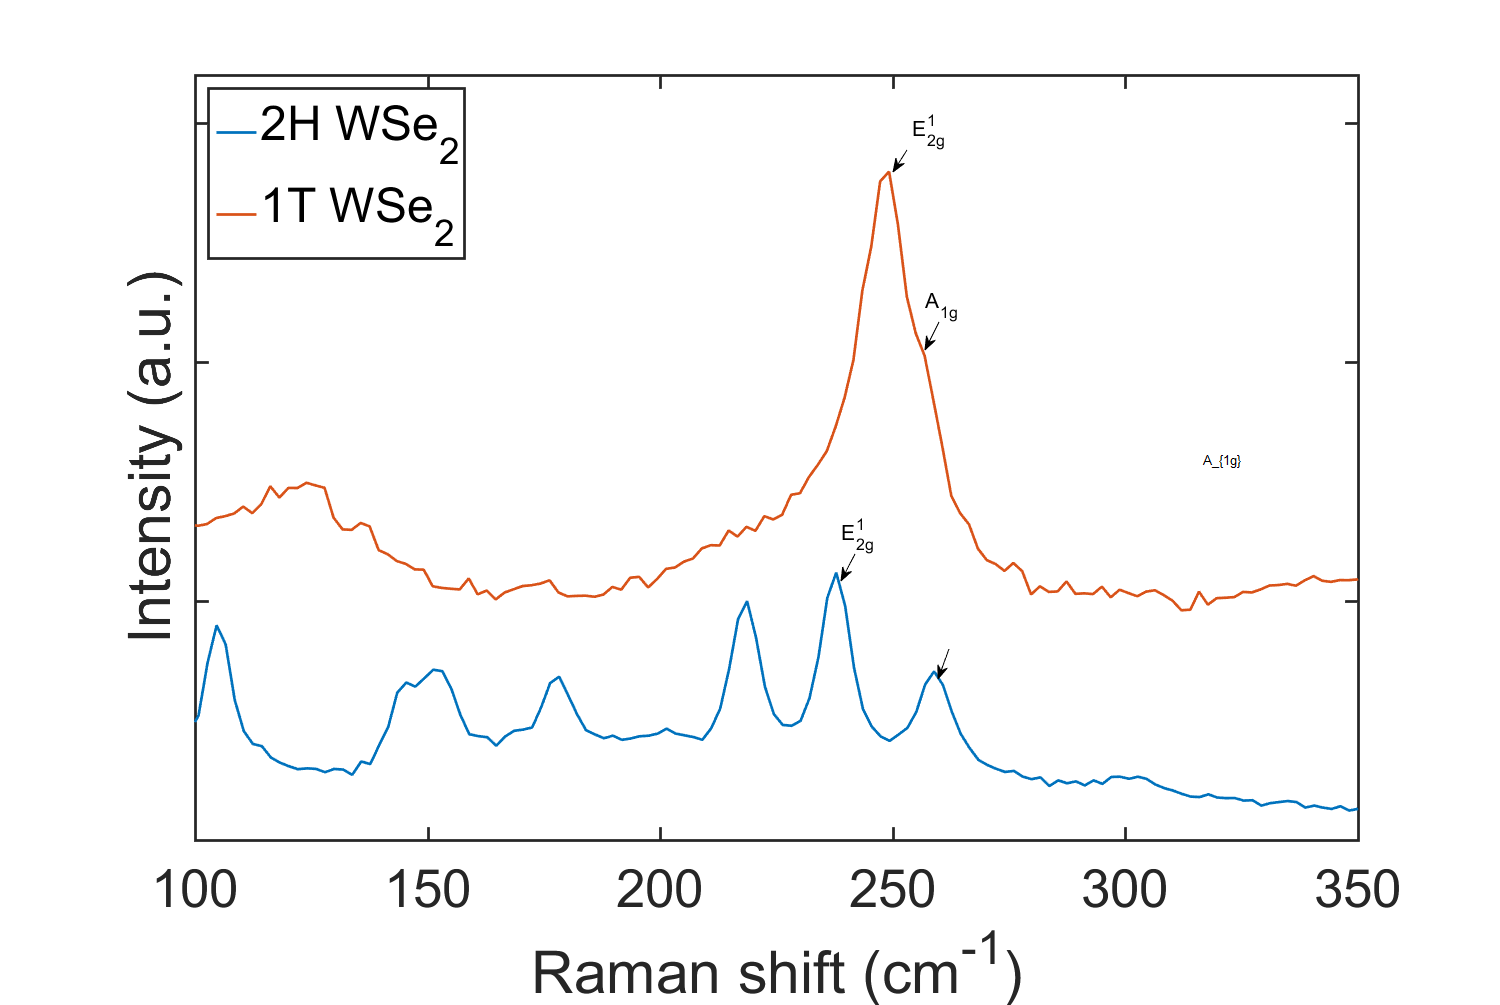
\includegraphics[scale=0.3]{1T'/RamanSpectraComparison.png}
		\caption{Raman spectra of 2H $WSe_2$ and 1T' $WSe_2$}
		\label{fig:1T'RamanSpectraComparison}
	\end{center}
\end{figure}

Similarly, the XPS spectra were taken of the as-grown sample as seen in Figure \ref{fig:1T'XPSW4fPreSpectrum} and Figure \ref{fig:1T'XPSSe3dPreSpectrum}. The XPS spectrum of the W 4f electron shell shows a doublet of $W^{+4}$ 4f at 31.49 and 33.63 eV. This position varies notably from those reported for 2H $WSe_2$ and therefore are attributed to 1T' $WSe_2$. The shift itself is most likely caused by change in coordination of the metal atom or a change in the W-Se bond length from 2.531 \r{A} to 2.66 \r{A}. On top of the 1T' phase of $WSe_2$ additional small contributions to the spectrum can be attributed to the 2H $WSe_2$ at 32.22 eV and 34.30 eV. Additionally an even smaller contribution from tungsten oxides can be identified at 35.74 eV and 37.92 eV. The Se 3d level spectrum seen in Figure \ref{fig:1T'XPSSe3dPreSpectrum} of the as-grown sample has been fitted with 4 doublets. Two of those doublets are associated with $Se^{-2}$ atoms and are assigned to 1T' $WSe_2$ (53.60 eV and 54.46 eV) and 2H $WSe_2$ (54.26 eV and 55.1 eV). The remaining two doublets, with much lower integrated area as compared to the Se bound to W, are assigned to amorphous Se (54.62 eV and 55.46 eV) and Se partially coordinated with phosphines (55.49 eV and 56.36 eV). The latter is remaining from the unreacted precursors of Se for the colloidal synthesis and a small component of amorphous Se is excepted as residual from the synthesis as well.

\begin{figure}[H]
	\begin{center}
		\begin{subfigure}[b]{0.7\textwidth}
			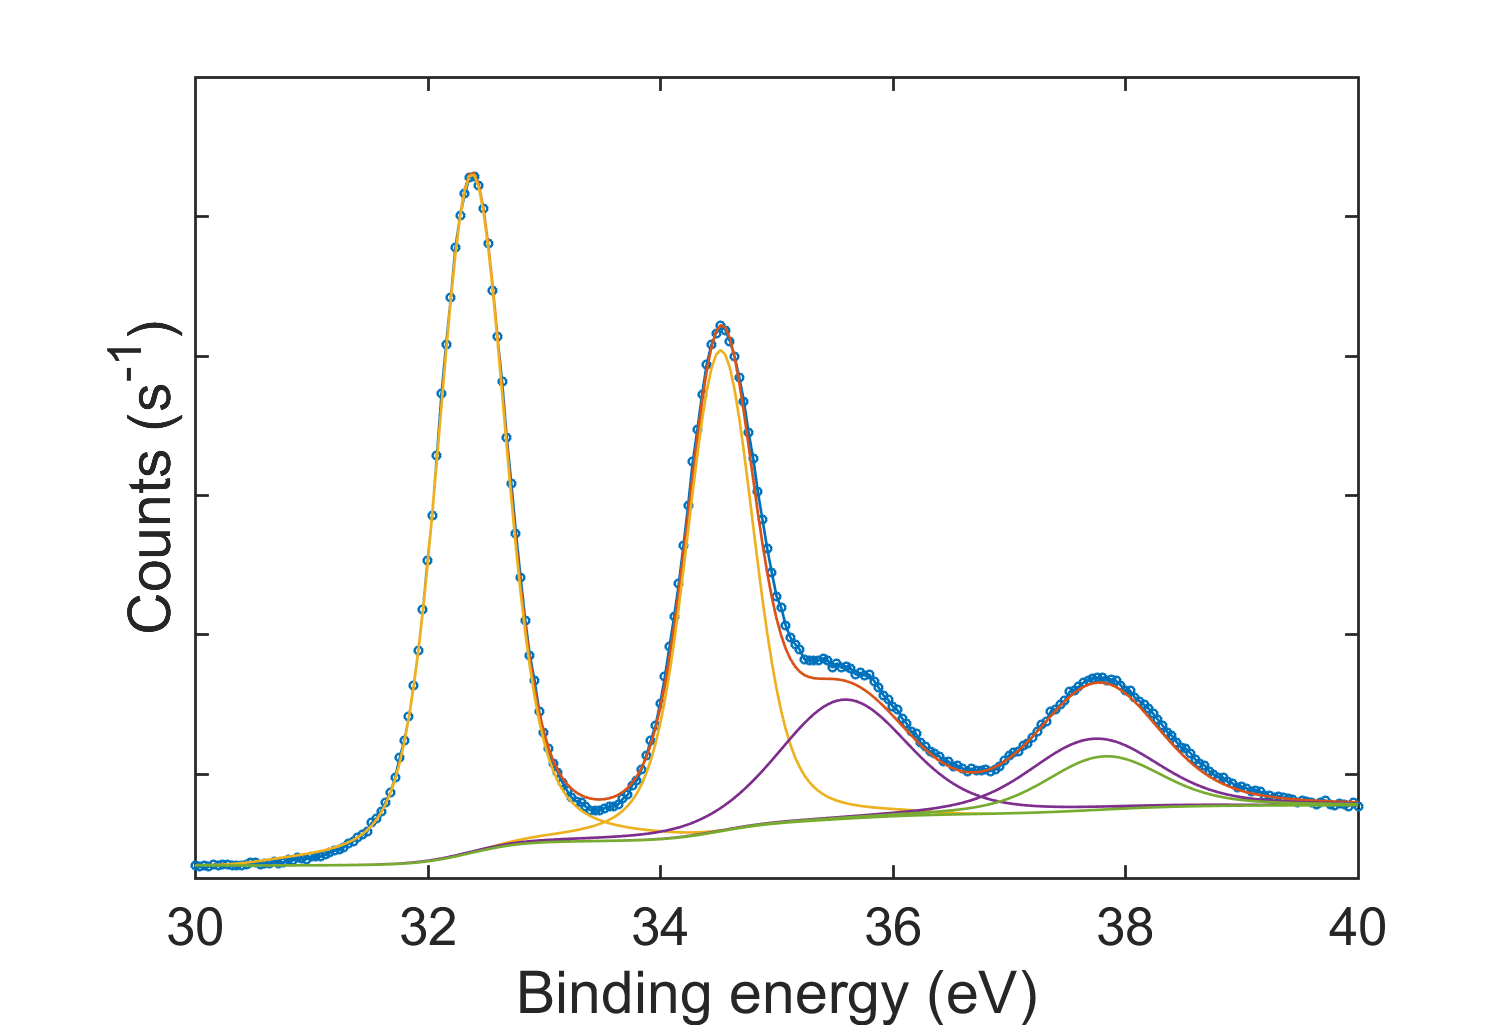
\includegraphics[width=\textwidth]{1T'/XPSW4fPre.png}
			\caption{W 4f}
			\label{fig:1T'XPSW4fPreSpectrum}
		\end{subfigure}
		\qquad
		\begin{subfigure}[b]{0.7\textwidth}
			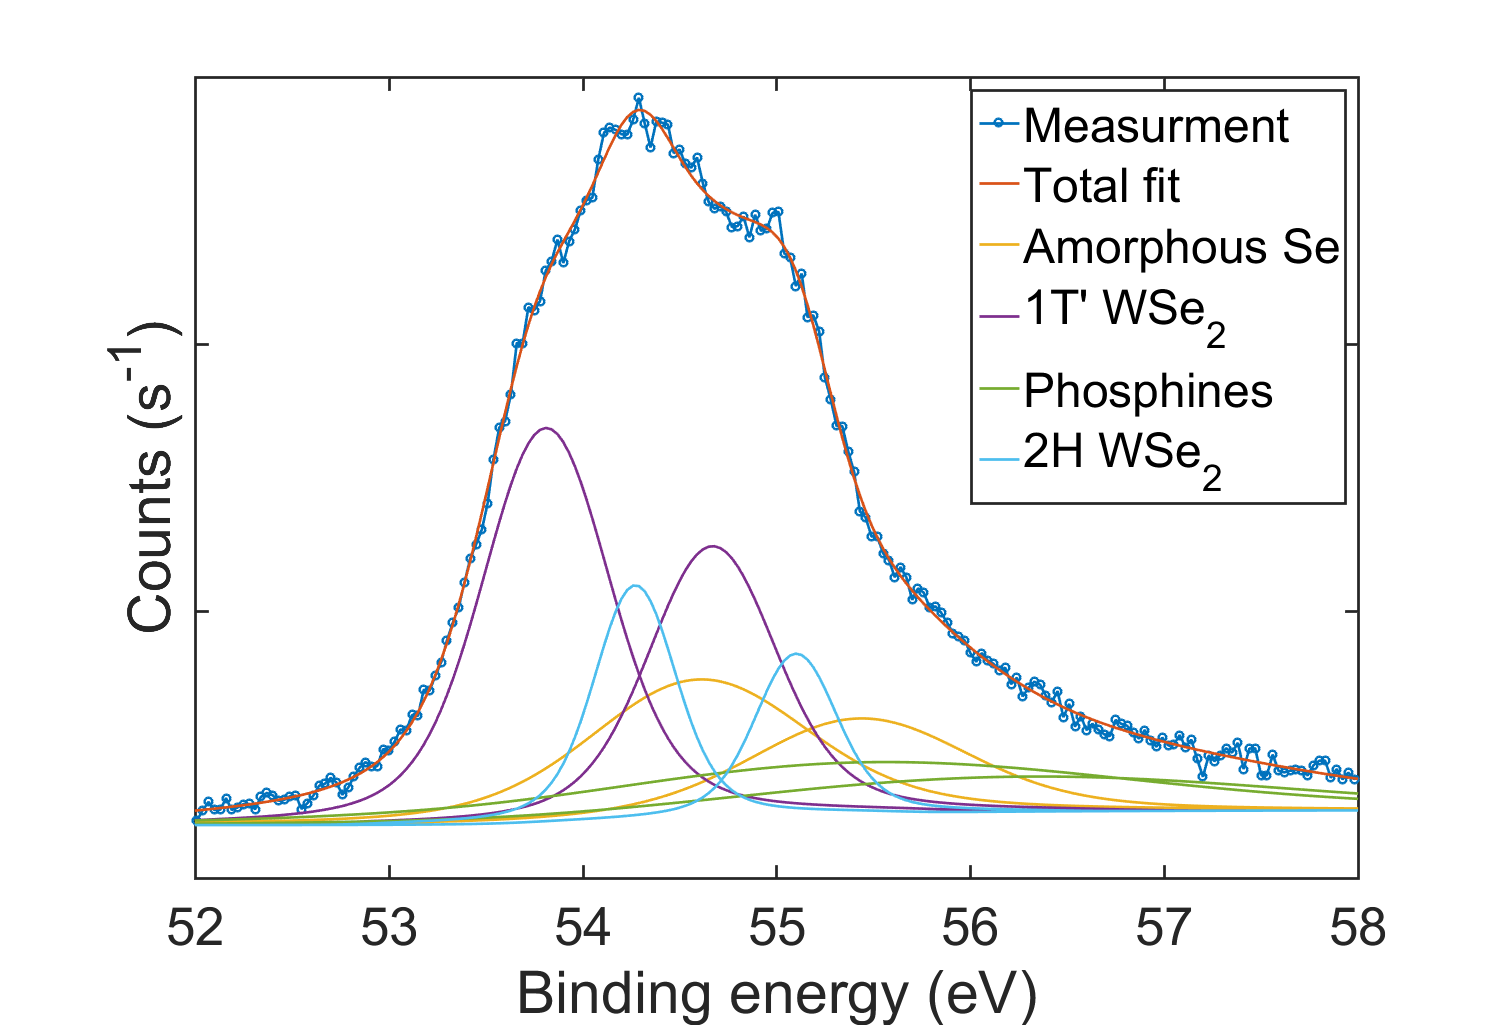
\includegraphics[width=\textwidth]{1T'/XPSSe3dPre.png}
			\caption{Se 3d}
			\label{fig:1T'XPSSe3dPreSpectrum}
		\end{subfigure}
		\caption{XPS spectra of W 4f and Se 3d levels in as grown sample of $WSe_2$}
		\label{fig:1T'XPSPreSpectra}
	\end{center}
\end{figure}

\begin{figure}[H]
	\begin{center}
		\begin{subfigure}[b]{0.7\textwidth}
			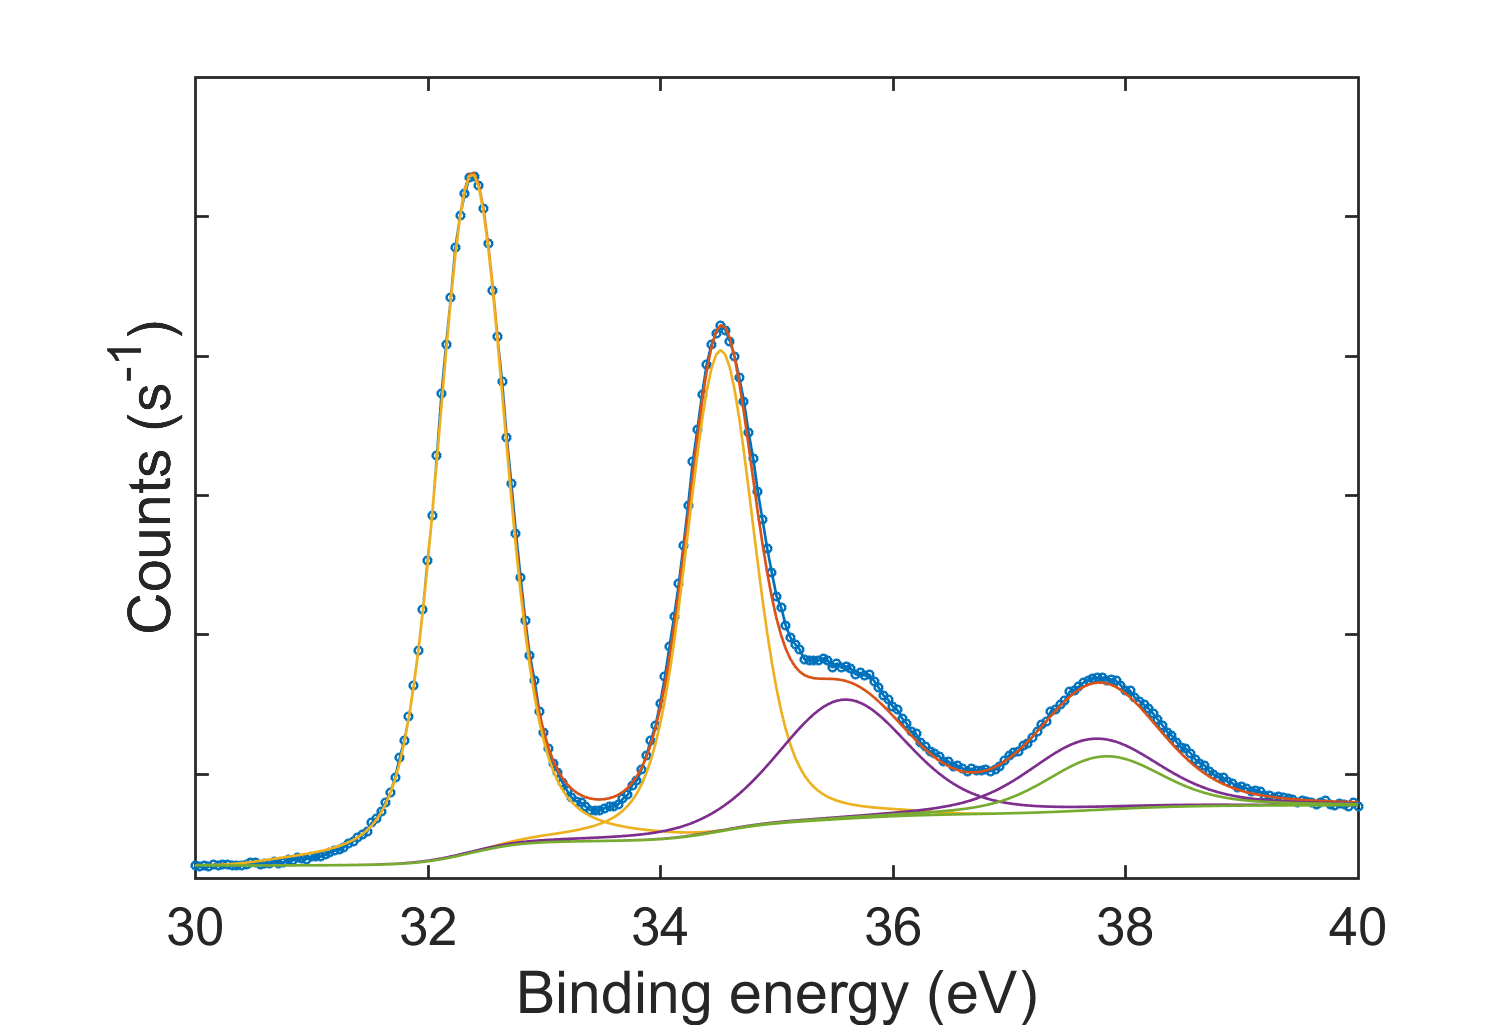
\includegraphics[width=\textwidth]{1T'/XPSW4fAnn.png}
			\caption{W 4f}
			\label{fig:1T'XPSW4fAnnSpectrum}
		\end{subfigure}
		\qquad
		\begin{subfigure}[b]{0.7\textwidth}
			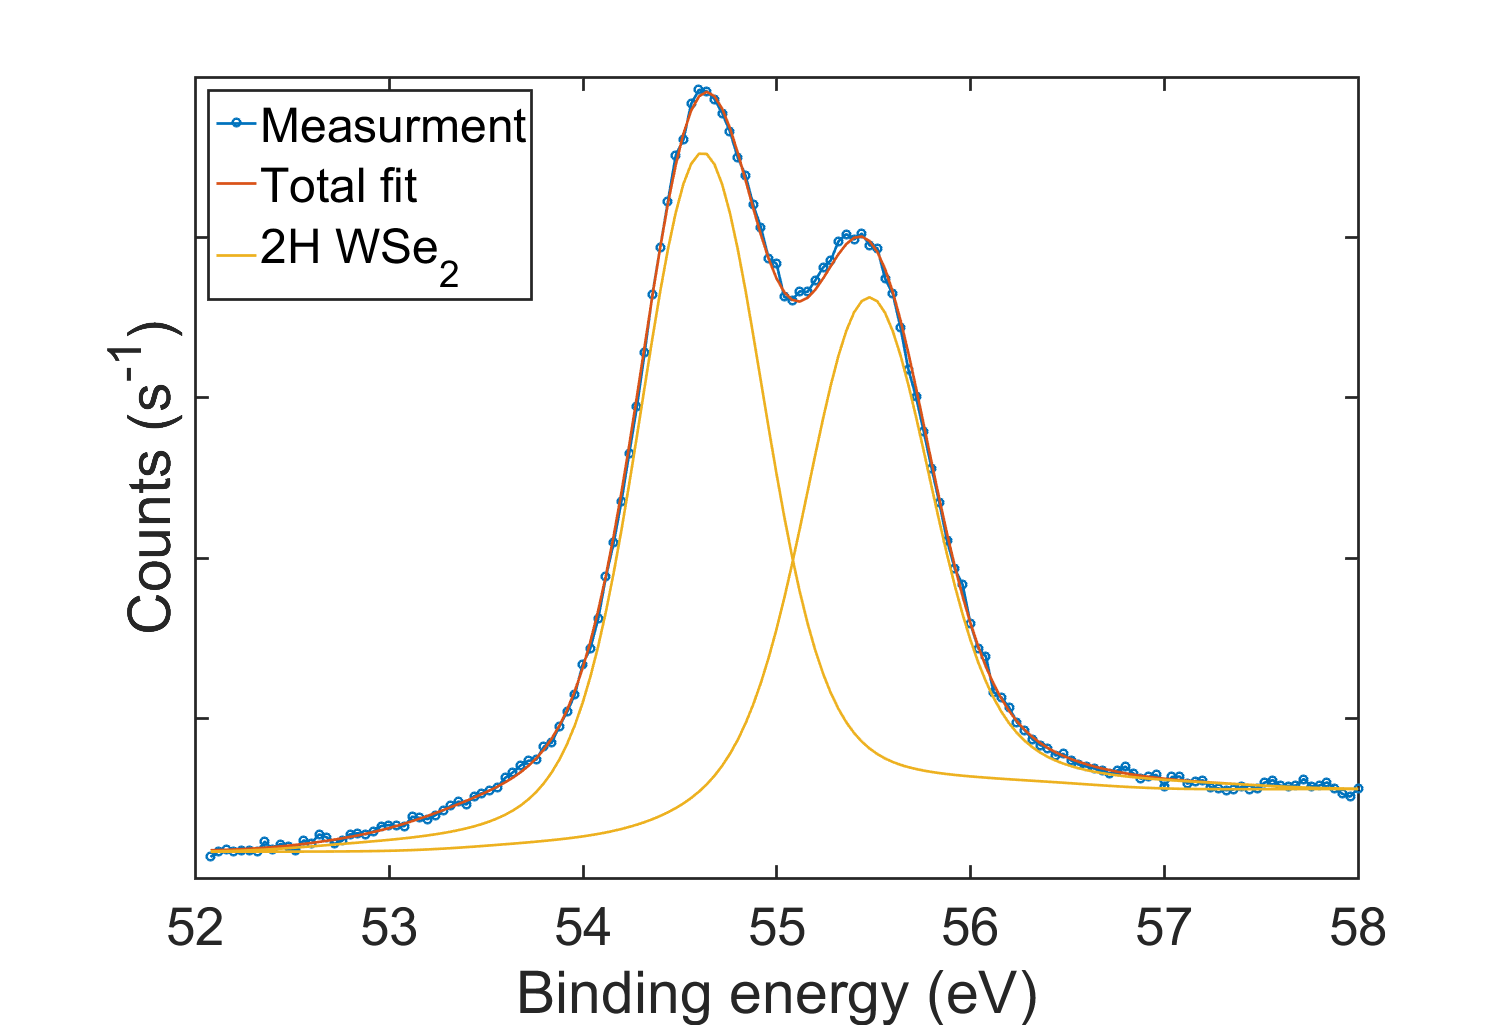
\includegraphics[width=\textwidth]{1T'/XPSSe3dAnn.png}
			\caption{Se 3d}
			\label{fig:1T'XPSSe3dAnnSpectrum}
		\end{subfigure}
		\caption{XPS spectra of W 4f and Se 3d levels in the annealed sample of $WSe_2$}
		\label{fig:1T'XPSAnnSpectra}
	\end{center}
\end{figure}

The as-grown sample was then annealed at 400 {\degree}C in an argon atmosphere. The Raman spectrum of the annealed sample can be seen in Figure \ref{fig:1T'RamanSpectraComparison}. The previously unidentified peaks are no longer present except for the two convoluted peaks at around 250 $cm^{-1}$. This is indicative of 2H $WSe_2$ and suggests that the entirety of the 1T' phase has been converted to the 2H phase. Additionally the XPS spectra of the annealed sample can be seen in Figure \ref{fig:1T'XPSAnnSpectra}. The presence of 4f $W^{4+}$ peaks 32.40 eV and 34.58 eV and an almost complete absence of the 1T' 4f $WSe_2$ indicates that the sample is primarily a 2H $WSe_2$. It is worth noting that after annealing the oxidized component of W just increases by a negligible amount. Following the annealing the XPS spectrum of the Se 3d can be seen in Figure \ref{fig:1T'XPSSe3dAnnSpectrum}. The spectrum can be fitted with one doublet associated with 2H $WSe_2$ only. This indicates that any residues of unreacted Se can be removed by annealing as expected as the evaporation temperature of elemental Se is $\sim$270 {\degree}C. 

\section{Conclusions}

In this chapter we have shown how the 1T' $WSe_2$ has been grown for the first time using this colloidal synthesis route. The material has then been characterised using Raman spectroscopy, XPS, TEM, and KPFM to ascertain to be in the 1T’ crystal phase and to demonstrate  to be metallic. Following an annealing at 400 {\degree}C the 1T' phase has been almost entirely converted to 2H. We have ascertain the presence of the 2H phase by preforming Raman spectroscopy, XPS, TEM, and characterization. This growth method therefore allows for direct deposition of metastable phase on a functional substrate. Our Raman and XPS characterization of the 1T’ phase represent a reference in the literature for future synthesis of 1T’ phases of TMDCs.